\documentclass[aspectratio=169,11pt]{beamer}

% ---- Minimalist theme ----
\usetheme{default}
\usecolortheme{default}
\setbeamertemplate{navigation symbols}{}
\setbeamertemplate{frametitle continuation}{}
\setbeamertemplate{itemize items}[circle]
\setbeamertemplate{enumerate items}[default]

% ---- Font: TeX Gyre Heros (clean Helvetica) ----
\usepackage[T1]{fontenc}
\usepackage{tgheros}
\renewcommand{\familydefault}{\sfdefault}
\usepackage{microtype}

% ---- Packages ----
\usepackage{amsmath}
\usepackage{booktabs}
\usepackage{tikz}
\usepackage{xcolor}
\usepackage{graphicx}
\usepackage{hyperref}
\usepackage{listings}

\usetikzlibrary{arrows.meta,positioning,calc,shapes.geometric,fit,decorations.pathreplacing}

% ---- Maastricht University Colors ----
\definecolor{umdark}{HTML}{001C3D}       % UM primary dark blue
\definecolor{umorange}{HTML}{E84E10}     % UM accent orange-red
\definecolor{umlight}{HTML}{4A90C4}      % UM light blue accent
\definecolor{umgray}{HTML}{6B7280}       % neutral gray
\definecolor{umbg}{HTML}{F8F9FA}         % very light background
\definecolor{umfaint}{HTML}{E5E7EB}      % faint rule color
\definecolor{umgreen}{HTML}{059669}      % success green

% ---- Apply UM colors to Beamer ----
\setbeamercolor{normal text}{fg=umdark}
\setbeamercolor{frametitle}{fg=umdark}
\setbeamercolor{title}{fg=umdark}
\setbeamercolor{subtitle}{fg=umgray}
\setbeamercolor{author}{fg=umgray}
\setbeamercolor{date}{fg=umgray}
\setbeamercolor{institute}{fg=umorange}
\setbeamercolor{itemize item}{fg=umorange}
\setbeamercolor{itemize subitem}{fg=umlight}
\setbeamercolor{enumerate item}{fg=umorange}
\setbeamercolor{block title}{bg=umdark,fg=white}
\setbeamercolor{block body}{bg=umdark!5,fg=umdark}
\setbeamercolor{block title alerted}{bg=umorange,fg=white}
\setbeamercolor{block body alerted}{bg=umorange!5,fg=umdark}
\setbeamercolor{block title example}{bg=umlight,fg=white}
\setbeamercolor{block body example}{bg=umlight!5,fg=umdark}

% ---- Code listing style ----
\lstset{
  basicstyle=\ttfamily\scriptsize,
  keywordstyle=\color{umdark}\bfseries,
  commentstyle=\color{umgray},
  stringstyle=\color{umorange},
  backgroundcolor=\color{umbg},
  frame=single,
  rulecolor=\color{umfaint},
  breaklines=true,
  showstringspaces=false
}

% ---- Frametitle with thin rule ----
\setbeamertemplate{frametitle}{%
  \vspace{0.35cm}%
  \noindent\hspace*{0pt}%
  \parbox{\textwidth}{%
    {\usebeamerfont{frametitle}\usebeamercolor[fg]{frametitle}\insertframetitle}%
    \vspace{2pt}\\%
    {\color{umorange}\rule{\textwidth}{1.2pt}}%
  }%
  \vspace{-2pt}%
}
\setbeamerfont{frametitle}{size=\large,series=\bfseries}
\setbeamersize{text margin left=0.7cm,text margin right=0.7cm}

% ---- Minimal footline ----
\setbeamertemplate{footline}{%
  \hbox{%
    \begin{beamercolorbox}[wd=\paperwidth,ht=2.2ex,dp=1ex]{footline}%
      \hspace{1em}{\scriptsize\color{umgray}Implementation Guide -- Image Steganography Study}%
      \hfill%
      {\scriptsize\color{umgray}\insertframenumber/\inserttotalframenumber}%
      \hspace{1em}%
    \end{beamercolorbox}%
  }%
}

% ---- Title ----
\title{Implementation Guide:\\Image Steganography Experiment}
\subtitle{Step-by-Step Technical Walkthrough}
\author{Nico \;\textbar\; Nikolas \;\textbar\; Abdul \;\textbar\; Daria \;\textbar\; Jimena \;\textbar\; David}
\institute{Department of Advanced Computing Sciences\\Maastricht University}
\date{Project 2.2\enspace\textbar\enspace February 2026}

\begin{document}

% ============================================================
% TITLE
% ============================================================
\begin{frame}[plain]
\vfill
\begin{center}
{\color{umorange}\rule{0.4\textwidth}{2pt}}\\[12pt]
{\LARGE\bfseries\color{umdark}\inserttitle}\\[10pt]
{\normalsize\color{umgray}\insertsubtitle}\\[16pt]
{\small\color{umdark}\insertauthor}\\[6pt]
{\small\color{umorange}\insertinstitute}\\[8pt]
{\footnotesize\color{umgray}\insertdate}\\[12pt]
{\color{umorange}\rule{0.4\textwidth}{2pt}}
\end{center}
\vfill
\end{frame}

% ============================================================
% OVERVIEW
% ============================================================
\begin{frame}{Implementation Overview}
\vspace{0.1cm}
\centering
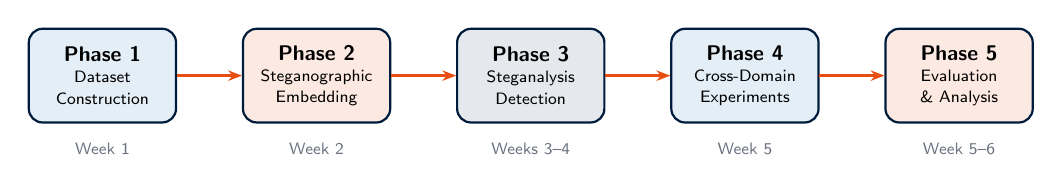
\begin{tikzpicture}[scale=0.85, every node/.style={scale=0.85},
  phase/.style={draw=umdark,rounded corners=5pt,minimum width=2.2cm,minimum height=1.4cm,align=center,font=\small,thick,fill=white},
  arr/.style={-{Stealth[length=5pt]},very thick,umorange}
]
\node[phase,fill=umlight!15] (p1) at (0,0) {\textbf{Phase 1}\\[-2pt]{\scriptsize Dataset}\\[-2pt]{\scriptsize Construction}};
\node[phase,fill=umorange!12] (p2) at (3.2,0) {\textbf{Phase 2}\\[-2pt]{\scriptsize Steganographic}\\[-2pt]{\scriptsize Embedding}};
\node[phase,fill=umdark!10] (p3) at (6.4,0) {\textbf{Phase 3}\\[-2pt]{\scriptsize Steganalysis}\\[-2pt]{\scriptsize Detection}};
\node[phase,fill=umlight!15] (p4) at (9.6,0) {\textbf{Phase 4}\\[-2pt]{\scriptsize Cross-Domain}\\[-2pt]{\scriptsize Experiments}};
\node[phase,fill=umorange!12] (p5) at (12.8,0) {\textbf{Phase 5}\\[-2pt]{\scriptsize Evaluation}\\[-2pt]{\scriptsize \& Analysis}};

\draw[arr] (p1) -- (p2);
\draw[arr] (p2) -- (p3);
\draw[arr] (p3) -- (p4);
\draw[arr] (p4) -- (p5);

\node[font=\scriptsize,text=umgray,below=4pt of p1] {Week 1};
\node[font=\scriptsize,text=umgray,below=4pt of p2] {Week 2};
\node[font=\scriptsize,text=umgray,below=4pt of p3] {Weeks 3--4};
\node[font=\scriptsize,text=umgray,below=4pt of p4] {Week 5};
\node[font=\scriptsize,text=umgray,below=4pt of p5] {Week 5--6};
\end{tikzpicture}

\vspace{0.3cm}

\begin{columns}[T]
\begin{column}{0.45\textwidth}
\begin{block}{Deliverables}
\small
\begin{itemize}
\item 1,000 images (500 real + 500 ML-generated)
\item Cover/stego pairs across all conditions
\item Steganalysis results (RS Analysis + SRM)
\item Statistical analysis + visualizations
\end{itemize}
\end{block}
\end{column}
\begin{column}{0.45\textwidth}
\begin{block}{Tech Stack}
\small
\begin{itemize}
\item Python 3.11+ with NumPy, SciPy
\item scikit-learn (SRM/FLD), Pillow, scikit-image
\item diffusers (Stable Diffusion), StyleGAN3
\item Matplotlib, Seaborn for plots
\end{itemize}
\end{block}
\end{column}
\end{columns}
\end{frame}

% ============================================================
% PHASE 1: DATASET
% ============================================================
\section{Phase 1: Dataset Construction}

\begin{frame}{Phase 1: Dataset Construction -- Overview}
\vspace{0.2cm}
\centering
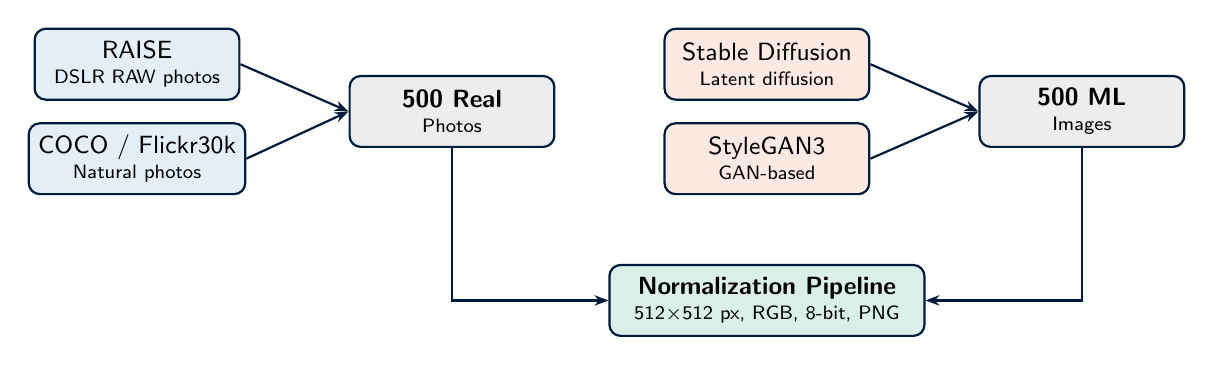
\begin{tikzpicture}[
  box/.style={draw=umdark,rounded corners=4pt,minimum width=2.6cm,minimum height=0.9cm,align=center,font=\small,thick},
  arr/.style={-{Stealth[length=5pt]},thick,umdark}
]
% Real branch
\node[box,fill=umlight!15] (raise) at (0,2) {RAISE\\[-2pt]{\scriptsize DSLR RAW photos}};
\node[box,fill=umlight!15] (coco) at (0,0.8) {COCO / Flickr30k\\[-2pt]{\scriptsize Natural photos}};
\node[box,fill=umdark!8] (real) at (4,1.4) {\textbf{500 Real}\\[-2pt]{\scriptsize Photos}};

% ML branch
\node[box,fill=umorange!12] (sd) at (8,2) {Stable Diffusion\\[-2pt]{\scriptsize Latent diffusion}};
\node[box,fill=umorange!12] (sg3) at (8,0.8) {StyleGAN3\\[-2pt]{\scriptsize GAN-based}};
\node[box,fill=umdark!8] (ml) at (12,1.4) {\textbf{500 ML}\\[-2pt]{\scriptsize Images}};

% Normalization
\node[box,fill=umgreen!15,minimum width=4cm] (norm) at (8,-1) {\textbf{Normalization Pipeline}\\[-2pt]{\scriptsize 512$\times$512 px, RGB, 8-bit, PNG}};

\draw[arr] (raise.east) -- (real.west);
\draw[arr] (coco.east) -- (real.west);
\draw[arr] (sd.east) -- (ml.west);
\draw[arr] (sg3.east) -- (ml.west);
\draw[arr] (real.south) |- (norm.west);
\draw[arr] (ml.south) |- (norm.east);
\end{tikzpicture}

\vspace{0.4cm}

\begin{alertblock}{Key Principle: Controlled Comparison}
\small
ML-generated images use the \textbf{same semantic prompts} derived from real image content (e.g., ``a dog in a park''). All images normalized to \textbf{identical specifications} to isolate carrier origin as the only variable.
\end{alertblock}
\end{frame}

% ---- Real Image Collection ----
\begin{frame}{Phase 1.1: Real Image Collection}
\begin{columns}[T]
\begin{column}{0.48\textwidth}
\begin{exampleblock}{RAISE Dataset}
\scriptsize
\textbf{Source:} High-quality RAW images from DSLR cameras [Dang-Nguyen et al., 2015]

\smallskip

\textbf{Characteristics:}
\begin{itemize}
\item Uncompressed RAW format, diverse scenes
\item Well-characterized, minimal processing artifacts
\item Ideal for steganography baseline (high SNR)
\end{itemize}

\smallskip

\textbf{Selection criteria:}
\begin{itemize}
\item Convert RAW $\rightarrow$ PNG at 512$\times$512
\item Balanced across scene categories
\end{itemize}
\end{exampleblock}
\end{column}

\begin{column}{0.48\textwidth}
\begin{block}{COCO / Flickr30k Supplement}
\scriptsize
\textbf{Purpose:} Add content and scene diversity

\smallskip

\textbf{Characteristics:}
\begin{itemize}
\item Natural everyday photographs
\item Rich semantic annotations (useful for prompt matching)
\item Widely used in CV research
\end{itemize}
\end{block}

\vspace{0.2cm}

\begin{block}{Sampling Strategy}
\scriptsize
\begin{itemize}
\item 250 images from RAISE
\item 250 images from COCO / Flickr30k
\item Stratified across scene categories
\item Extract semantic captions for ML matching
\end{itemize}
\end{block}
\end{column}
\end{columns}
\end{frame}

% ---- ML Image Generation ----
\begin{frame}{Phase 1.2: ML Image Generation}
\begin{columns}[T]
\begin{column}{0.48\textwidth}
\begin{block}{Stable Diffusion (v2.1)}
\scriptsize
\textbf{Architecture:} Latent diffusion model (LDM) [Rombach et al., 2022]

\smallskip

\textbf{Key features:}
\begin{itemize}
\item Text-to-image from semantic prompts
\item Produces photorealistic results
\item Runs locally via \texttt{diffusers} library (MPS)
\item $\sim$3--5 hours for 250 images
\end{itemize}

\smallskip

\textbf{Generation parameters:}
\begin{itemize}
\item Guidance scale: 7.5 (balanced quality)
\item Steps: 50 (DDIM sampler)
\item Prompts derived from real image captions
\item Output: PNG, 512$\times$512
\end{itemize}
\end{block}
\end{column}

\begin{column}{0.48\textwidth}
\begin{block}{StyleGAN3}
\scriptsize
\textbf{Architecture:} Alias-free GAN [Karras et al., 2021]

\smallskip

\textbf{Key features:}
\begin{itemize}
\item Well-characterized spectral artifacts (GAN fingerprint)
\item High-resolution, diverse outputs
\item Official NVIDIA PyTorch implementation
\item $\sim$2--3 hours for 250 images
\end{itemize}

\smallskip

\textbf{Generation parameters:}
\begin{itemize}
\item Use pretrained FFHQ or LSUN checkpoint
\item Truncation: $\psi = 0.7$ (diversity vs.\ quality)
\item Output: PNG, 512$\times$512
\end{itemize}
\end{block}
\end{column}
\end{columns}

\vspace{0.15cm}

\centering
{\scriptsize\color{umgray}\textbf{Optional extension:} DALL-E 3 via API as a third generation source (time permitting)}
\end{frame}

% ---- Normalization Pipeline ----
\begin{frame}{Phase 1.3: Image Normalization Pipeline}
\begin{columns}[T]
\begin{column}{0.55\textwidth}
\begin{block}{Normalization Steps}
\scriptsize
\begin{enumerate}
\item \textbf{Decode / convert:} RAW $\rightarrow$ RGB (dcraw or rawpy); generated images already PNG
\item \textbf{Resize:} Center-crop and resize to 512$\times$512 pixels (Lanczos)
\item \textbf{Color space:} Ensure sRGB color space
\item \textbf{Bit depth:} Convert to 8-bit per channel (uint8)
\item \textbf{Luminance:} Normalize mean luminance across dataset
\item \textbf{Format:} Export as lossless PNG (no JPEG compression artifacts)
\end{enumerate}
\end{block}

\vspace{0.1cm}

\begin{alertblock}{Quality Gate}
\scriptsize
Reject images with BRISQUE score $>$ 50 (poor perceptual quality). Re-generate rejected ML images with different seeds.
\end{alertblock}
\end{column}

\begin{column}{0.40\textwidth}
\centering
\scriptsize
\begin{tabular}{@{}ll@{}}
\toprule
\textbf{Parameter} & \textbf{Value} \\
\midrule
Dimensions & 512$\times$512 px \\
Color space & RGB (sRGB) \\
Bit depth & 8-bit/channel \\
Channels & 3 (RGB) \\
Format & PNG (lossless) \\
\bottomrule
\end{tabular}

\vspace{0.3cm}

\begin{block}{\small File Naming Convention}
\scriptsize
\texttt{<source>\_<id>\_<category>.png}\\[2pt]
\texttt{real\_001\_cat042.png}\\
\texttt{sd\_001\_cat042.png}\\
\texttt{sg3\_001\_cat042.png}
\end{block}
\end{column}
\end{columns}
\end{frame}

% ============================================================
% PHASE 2: EMBEDDING
% ============================================================
\section{Phase 2: Steganographic Embedding}

\begin{frame}{Phase 2: Steganographic Embedding -- Overview}
\vspace{0.1cm}

\begin{block}{Embedding Methods}
\scriptsize
We implement two complementary methods spanning the capacity--imperceptibility trade-off, each applied with and without AES-256 payload encryption:
\end{block}

\vspace{0.2cm}

\begin{columns}[T]
\begin{column}{0.46\textwidth}
\begin{exampleblock}{LSB Substitution (Spatial Domain)}
\scriptsize
\textbf{Principle:} Replace least significant bits of pixel channel values with message bits.

\smallskip

\textbf{Characteristics:}
\begin{itemize}
\item High embedding capacity
\item Simple implementation (NumPy / Pillow)
\item Vulnerable to statistical attacks
\item Detectable via histogram analysis [Fridrich et al., 2001]
\end{itemize}
\end{exampleblock}
\end{column}

\begin{column}{0.46\textwidth}
\begin{block}{DCT-Based Embedding (Freq. Domain)}
\scriptsize
\textbf{Principle:} Modify DCT coefficients of 8$\times$8 pixel blocks using QIM [Chen \& Wornell, 2001].

\smallskip

\textbf{Characteristics:}
\begin{itemize}
\item Better imperceptibility
\item Mirrors JPEG-domain steganography (F5)
\item Lower capacity than LSB
\item Targets mid-frequency coefficients
\end{itemize}
\end{block}
\end{column}
\end{columns}

\vspace{0.15cm}

\centering
{\scriptsize\color{umgray}Both methods use \textbf{pseudorandom pixel/coefficient selection} keyed by a shared secret. Payload optionally pre-encrypted with \textbf{AES-256-CBC}.}
\end{frame}

% ---- LSB Implementation ----
\begin{frame}{Phase 2.1: LSB Embedding Implementation}
\begin{columns}[T]
\begin{column}{0.52\textwidth}
\begin{block}{Algorithm}
\scriptsize
\begin{enumerate}
\item \textbf{Input:} Cover image $\mathbf{I}$ (H$\times$W$\times$3), message $\mathbf{m}$, key $K$, params $(k, p)$
\item \textbf{(Optional) Encrypt:} $\mathbf{m} \leftarrow \text{AES-256}(\mathbf{m}, K_\text{aes})$
\item \textbf{Generate mask:} PRNG seeded with $K$ selects $p\%$ of pixels (all 3 channels)
\item \textbf{For each selected pixel channel $I_{ij}^c$:}
  \begin{itemize}
  \item Replace $k$ LSBs: $I_{ij}^{c\prime} = (I_{ij}^c \land \overline{M_k}) \lor m_{bits}$
  \end{itemize}
\item \textbf{Output:} Stego image $\mathbf{I}'$, saved as lossless PNG
\end{enumerate}
\end{block}

\vspace{0.1cm}

\begin{alertblock}{Message Preparation}
\scriptsize
Pseudorandom bit sequence (deterministic via seed) as payload; ensures reproducibility and content-independence.
\end{alertblock}
\end{column}

\begin{column}{0.44\textwidth}
\centering
\scriptsize
\begin{tabular}{@{}llr@{}}
\toprule
\textbf{Level} & \textbf{Config} & \textbf{bpp} \\
\midrule
Low      & $k\!=\!1$, 25\% px & $\sim$0.08 \\
Medium   & $k\!=\!1$, 50\% px & $\sim$0.16 \\
High     & $k\!=\!2$, 50\% px & $\sim$0.32 \\
\bottomrule
\end{tabular}

\vspace{0.1cm}
{\scriptsize bpp = bits per pixel}

\vspace{0.3cm}

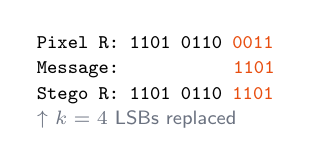
\begin{tikzpicture}[scale=0.75]
\node[font=\scriptsize\ttfamily,anchor=west] at (0,0.9) {Pixel R: 1101 0110 \textcolor{umorange}{0011}};
\node[font=\scriptsize\ttfamily,anchor=west] at (0,0.45) {Message:\hspace{1.45cm}\textcolor{umorange}{1101}};
\node[font=\scriptsize\ttfamily,anchor=west] at (0,0) {Stego R: 1101 0110 \textcolor{umorange}{1101}};
\node[font=\scriptsize,text=umgray,anchor=west] at (0,-0.4) {$\uparrow$ $k=4$ LSBs replaced};
\end{tikzpicture}
\end{column}
\end{columns}
\end{frame}

% ---- DCT Implementation ----
\begin{frame}{Phase 2.2: DCT Embedding Implementation}
\begin{columns}[T]
\begin{column}{0.52\textwidth}
\begin{block}{Algorithm (QIM-based) [Chen \& Wornell, 2001]}
\scriptsize
\begin{enumerate}
\item \textbf{(Optional) Encrypt:} $\mathbf{m} \leftarrow \text{AES-256}(\mathbf{m}, K_\text{aes})$
\item \textbf{Split into blocks:} Divide each channel into 8$\times$8 pixel blocks
\item \textbf{Apply 2D DCT:} $\mathbf{C} = \text{DCT2}(\mathbf{block})$
\item \textbf{Select coefficients:} Mid-frequency range via zigzag scan (positions 10--54 of 64)
\item \textbf{For each selected coefficient $C_i$:}
  \begin{itemize}
  \item Quantize and embed: $C_i' = \Delta \cdot \lfloor C_i / \Delta + 0.5 \rfloor \pm \Delta/4$ based on bit $b$
  \end{itemize}
\item \textbf{Inverse DCT:} $\mathbf{block}' = \text{IDCT2}(\mathbf{C}')$
\item \textbf{Reconstruct image:} Reassemble blocks, clip to [0, 255], save PNG
\end{enumerate}
\end{block}

{\scriptsize\color{umgray}$\Delta$ (quantization step) controls the capacity--imperceptibility trade-off.}
\end{column}

\begin{column}{0.44\textwidth}
\centering
\scriptsize
\begin{tabular}{@{}llr@{}}
\toprule
\textbf{Level} & \textbf{Coefficients} & \textbf{bpp} \\
\midrule
Low      & 10\% & $\sim$0.02 \\
Medium   & 25\% & $\sim$0.05 \\
High     & 50\% & $\sim$0.10 \\
\bottomrule
\end{tabular}

\vspace{0.25cm}

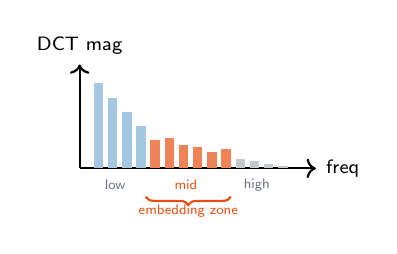
\begin{tikzpicture}[scale=0.6]
% Frequency axis
\draw[->,thick] (0,0) -- (5,0) node[right,font=\scriptsize] {freq};
\draw[->,thick] (0,0) -- (0,2.2) node[above,font=\scriptsize] {DCT mag};

% Bars representing DCT coefficients
\foreach \x/\h in {0.3/1.8, 0.6/1.5, 0.9/1.2, 1.2/0.9} {
  \fill[umlight!50] (\x,0) rectangle (\x+0.2,\h);
}
\foreach \x/\h in {1.5/0.6, 1.8/0.65, 2.1/0.5, 2.4/0.45, 2.7/0.35, 3.0/0.40} {
  \fill[umorange!70] (\x,0) rectangle (\x+0.2,\h);
}
\foreach \x/\h in {3.3/0.20, 3.6/0.15, 3.9/0.10, 4.2/0.06} {
  \fill[umgray!40] (\x,0) rectangle (\x+0.2,\h);
}

\node[font=\tiny,text=umgray] at (0.75,-0.35) {low};
\node[font=\tiny,text=umorange] at (2.25,-0.35) {mid};
\node[font=\tiny,text=umgray] at (3.75,-0.35) {high};

\draw[decorate,decoration={brace,amplitude=3pt,mirror},thick,umorange] (1.4,-0.6) -- (3.2,-0.6);
\node[font=\tiny,text=umorange] at (2.3,-0.9) {embedding zone};
\end{tikzpicture}
\end{column}
\end{columns}
\end{frame}

% ---- Embedding Pipeline ----
\begin{frame}{Phase 2.3: Complete Embedding Pipeline}
\vspace{0.1cm}
\centering
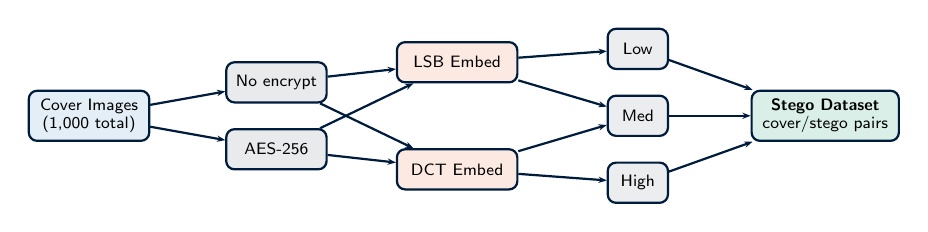
\begin{tikzpicture}[scale=0.85, every node/.style={scale=0.85},
  box/.style={draw=umdark,rounded corners=3pt,minimum width=1.8cm,minimum height=0.6cm,align=center,font=\scriptsize,thick},
  arr/.style={-{Stealth[length=3pt]},thick,umdark}
]
% Input
\node[box,fill=umlight!15] (cover) at (0,0) {Cover Images\\(1,000 total)};

% Encryption branch
\node[box,fill=umgray!15,minimum width=1.5cm] (plain) at (2.8,0.5) {No encrypt};
\node[box,fill=umgray!15,minimum width=1.5cm] (enc) at (2.8,-0.5) {AES-256};

% Embedding methods
\node[box,fill=umorange!12] (lsb) at (5.5,0.8) {LSB Embed};
\node[box,fill=umorange!12] (dct) at (5.5,-0.8) {DCT Embed};

% Payload levels
\node[box,fill=umdark!8,minimum width=0.9cm] (l1) at (8.2,1.0) {Low};
\node[box,fill=umdark!8,minimum width=0.9cm] (l2) at (8.2,0.0) {Med};
\node[box,fill=umdark!8,minimum width=0.9cm] (l3) at (8.2,-1.0) {High};

% Output
\node[box,fill=umgreen!15,minimum width=2.2cm] (stego) at (11,0) {\textbf{Stego Dataset}\\cover/stego pairs};

\draw[arr] (cover) -- (plain);
\draw[arr] (cover) -- (enc);
\draw[arr] (plain) -- (lsb);
\draw[arr] (enc) -- (lsb);
\draw[arr] (plain) -- (dct);
\draw[arr] (enc) -- (dct);
\draw[arr] (lsb) -- (l1);
\draw[arr] (lsb) -- (l2);
\draw[arr] (dct) -- (l2);
\draw[arr] (dct) -- (l3);
\draw[arr] (l1) -- (stego);
\draw[arr] (l2) -- (stego);
\draw[arr] (l3) -- (stego);
\end{tikzpicture}

\vspace{0.2cm}

\begin{columns}[T]
\begin{column}{0.32\textwidth}
\begin{block}{\small Conditions}
\scriptsize
1,000 covers $\times$ 2 methods $\times$ 3 payload levels $\times$ 2 encryption states = \textbf{12,000 stego images} (+ 1,000 covers = 13,000 total)
\end{block}
\end{column}

\begin{column}{0.32\textwidth}
\begin{block}{\small Quality Checks}
\scriptsize
Compute for each stego image:
\begin{itemize}
\item \textbf{PSNR}: target $>$ 40 dB
\item \textbf{SSIM}: target $>$ 0.95
\item \textbf{BER}: target = 0 (lossless PNG)
\end{itemize}
\end{block}
\end{column}

\begin{column}{0.32\textwidth}
\begin{block}{\small Storage Format}
\scriptsize
\texttt{stego/<source>/<method>/}\\
\texttt{\ \ <enc>/<level>/<id>.png}\\[4pt]
e.g.\ \texttt{stego/real/lsb/plain/}\\
\texttt{\ \ \ \ high/real\_042.png}
\end{block}
\end{column}
\end{columns}
\end{frame}

% ============================================================
% PHASE 3: DETECTION
% ============================================================
\section{Phase 3: Steganalysis Detection}

\begin{frame}{Phase 3: Steganalysis Detectors -- Overview}
\vspace{0.1cm}

\begin{block}{Detection Task}
\scriptsize
Binary detection: Given an image, determine whether it contains hidden data (\textbf{stego}) or is clean (\textbf{cover}). We use \textbf{classical signal processing methods only} — no neural networks, no GPUs.
\end{block}

\vspace{0.2cm}

\begin{columns}[T]
\begin{column}{0.30\textwidth}
\begin{exampleblock}{Chi-Square Attack [Westfeld \& Pfitzmann, 1999]}
\scriptsize
\textbf{Type:} Training-free statistical test

\smallskip

\textbf{Principle:}
\begin{itemize}
\item LSB embedding equalises histogram pair frequencies $(2k, 2k+1)$
\item Chi-square test detects this distribution shift
\item Returns a $p$-value and embedding probability estimate
\end{itemize}

\smallskip

\textbf{Strength:} Zero training, analytical, fast. Best for spatial-domain (LSB).
\end{exampleblock}
\end{column}

\begin{column}{0.30\textwidth}
\begin{block}{RS Analysis [Fridrich et al., 2001]}
\scriptsize
\textbf{Type:} Training-free statistical estimator

\smallskip

\textbf{Principle:}
\begin{itemize}
\item Groups pixels, classifies as Regular/Singular by smoothness function
\item LSB flipping shifts Regular/Singular/Negative counts predictably
\item Estimates payload rate $\hat{p}$ analytically from group counts
\end{itemize}

\smallskip

\textbf{Strength:} Generalizes to partial embedding; domain-agnostic by construction.
\end{block}
\end{column}

\begin{column}{0.30\textwidth}
\begin{block}{SRM + FLD Ensemble [Fridrich \& Kodovský, 2012]}
\scriptsize
\textbf{Type:} Classical ML (not neural network)

\smallskip

\textbf{Principle:}
\begin{itemize}
\item Extract $\sim$35,000 high-pass residual co-occurrence features
\item Ensemble of Fisher Linear Discriminants classifies cover vs.\ stego
\item CPU-only; fast ($\sim$30 min total)
\end{itemize}

\smallskip

\textbf{Strength:} Handles both LSB and DCT embedding; cross-domain generalization test.
\end{block}
\end{column}
\end{columns}
\end{frame}

% ---- RS Analysis ----
\begin{frame}{Phase 3.1: RS Analysis -- Algorithm}
\vspace{0.1cm}
\begin{columns}[T]
\begin{column}{0.52\textwidth}
\begin{block}{Algorithm [Fridrich, Goljan \& Du, 2001]}
\scriptsize
\begin{enumerate}
\item \textbf{Partition} image into disjoint pixel groups $G$ of size $n$ (e.g., $n=4$ horizontal)
\item \textbf{Define} discrimination function $f(G)$ = mean absolute difference between adjacent pixels
\item \textbf{Apply} flipping mask $M$ (toggles LSB) and its negative $-M$:
  \begin{itemize}
  \item $R_M$ = fraction of groups where $f(F_M(G)) > f(G)$ (Regular)
  \item $S_M$ = fraction of groups where $f(F_M(G)) < f(G)$ (Singular)
  \item $R_{-M}$, $S_{-M}$ = same with $F_{-M}$
  \end{itemize}
\item \textbf{Solve} quadratic equation for payload estimate:
  $$\hat{p} \approx \frac{2(R_{-M} - R_M)}{(R_{-M} - R_M) + (S_{-M} - S_M)}$$
\end{enumerate}
\end{block}
\end{column}

\begin{column}{0.44\textwidth}
\begin{exampleblock}{Key Properties}
\scriptsize
\begin{itemize}
\item \textbf{No training data} -- purely analytical
\item \textbf{Quantitative:} returns $\hat{p} \in [0,1]$; threshold at $\hat{p} > 0.01$
\item \textbf{Domain-agnostic:} same formula for real or ML-generated images
\item Runs in \textbf{seconds per image} with NumPy
\end{itemize}
\end{exampleblock}

\vspace{0.2cm}

\begin{block}{Why RS Analysis for Cross-Domain?}
\scriptsize
Since RS Analysis uses no training data, any difference in $\hat{p}$ between real and ML-generated carriers is purely due to the carriers' statistical properties — \textbf{not classifier bias}. This makes it the cleanest test of our primary hypothesis.
\end{block}
\end{column}
\end{columns}
\end{frame}

% ---- SRM ----
\begin{frame}{Phase 3.2: SRM + FLD Ensemble -- Algorithm}
\begin{columns}[T]
\begin{column}{0.52\textwidth}
\begin{block}{SRM Feature Extraction [Fridrich \& Kodovský, 2012]}
\scriptsize
\begin{enumerate}
\item \textbf{Apply} a bank of high-pass filters (e.g., 3$\times$3 SQUARE, EDGE kernels) to suppress image content and amplify residuals
\item \textbf{Quantize} residuals to small integer values (truncation)
\item \textbf{Compute} co-occurrence histograms from quantized residuals across multiple directions (horizontal, vertical, diagonal)
\item \textbf{Concatenate} all histograms into a $\sim$35,000-dimensional feature vector per image
\end{enumerate}

\smallskip

\textbf{Classification: Fisher Linear Discriminant (FLD) Ensemble}
\begin{itemize}
\item Train ensemble of binary FLD classifiers on feature subsets
\item Aggregate predictions by majority vote
\item Implementation: \texttt{sklearn.linear\_model.SGDClassifier}
\end{itemize}
\end{block}
\end{column}

\begin{column}{0.44\textwidth}
\begin{block}{Training Protocol}
\scriptsize
\begin{itemize}
\item \textbf{Folds:} 3-fold cross-validation (stratified by source)
\item \textbf{Input:} cover/stego image pairs
\item \textbf{Labels:} 0 = cover, 1 = stego
\item \textbf{Runtime:} $\sim$30 min total (CPU)
\end{itemize}
\end{block}

\vspace{0.2cm}

\begin{exampleblock}{Why SRM for Cross-Domain?}
\scriptsize
SRM's hand-crafted features are not tied to learned representations, making them \textbf{more likely to generalize} across real/ML domain boundary than neural networks would. Cross-domain conditions (C, D) test this directly.
\end{exampleblock}

\vspace{0.1cm}

\begin{alertblock}{Compute}
\scriptsize
\textbf{No GPU required.} All feature extraction and classification runs on CPU. Total SRM training: $\sim$54 runs $\times$ $\sim$30 sec = \textbf{$<$30 min}.
\end{alertblock}
\end{column}
\end{columns}
\end{frame}

% ============================================================
% PHASE 4: EXPERIMENTS
% ============================================================
\section{Phase 4: Cross-Domain Experiments}

\begin{frame}{Phase 4: Cross-Domain Experimental Conditions}
\begin{block}{Core Question [RQ4]}
\scriptsize
Do steganalysis classifiers trained on one domain (real or ML-generated images) generalize to the other?
\end{block}

\vspace{0.1cm}

\centering
\scriptsize
\begin{tabular}{@{}clllp{4.8cm}@{}}
\toprule
\textbf{Cond.} & \textbf{Train} & \textbf{Test} & \textbf{Addresses} & \textbf{Research Significance} \\
\midrule
\textbf{A} & Real & Real & Baseline & Standard steganalysis benchmark \\
\textbf{B} & ML-gen & ML-gen & Primary RQ & Is ML imagery easier/harder to steganalyze? \\
\textbf{C} & Real & ML-gen & RQ4, H5 & Real-trained detectors vs.\ synthetic carriers \\
\textbf{D} & ML-gen & Real & RQ4, H5 & ML-trained detectors vs.\ real images \\
\midrule
\textbf{E} & Mixed & Both & Mitigation & Domain-agnostic training \\
\bottomrule
\end{tabular}

\vspace{0.2cm}

\begin{columns}[T]
\begin{column}{0.48\textwidth}
\begin{alertblock}{Security Implication}
\scriptsize
If \textbf{C} shows poor performance, adversaries could evade real-world detectors simply by using ML-generated images as carriers.
\end{alertblock}
\end{column}
\begin{column}{0.48\textwidth}
\begin{exampleblock}{Expected Outcome [H4]}
\scriptsize
10--25\% AUC degradation in cross-domain conditions (C, D) vs.\ within-domain (A, B), paralleling findings in image deepfake detection [Wang et al., 2020].
\end{exampleblock}
\end{column}
\end{columns}
\end{frame}

% ---- Experiment Matrix ----
\begin{frame}{Phase 4.1: Full Experiment Matrix}
\vspace{0.1cm}
\centering
\tiny
\begin{tabular}{@{}lllllll@{}}
\toprule
\textbf{Detector} & \textbf{Training?} & \textbf{Method} & \textbf{Payload} & \textbf{Encryption} & \textbf{Condition} & \textbf{\# Runs} \\
\midrule
RS Analysis & None & LSB & Low, Med, High & Plain, AES & A--E (all) & $1\times3\times2\times5 = 30$ \\
Chi-square & None & LSB & Low, Med, High & Plain, AES & A--E (all) & $30$ \\
SRM + FLD & 3-fold CV & LSB & Low, Med, High & Plain, AES & A, B, C, D, E & $30$ \\
SRM + FLD & 3-fold CV & DCT & Low, Med, High & Plain, AES & A, B, C, D, E & $30$ \\
\midrule
\multicolumn{6}{r}{\textbf{Total unique configurations:}} & \textbf{120} \\
\multicolumn{6}{r}{\textbf{SRM training runs ($\times$3-fold):}} & \textbf{$\sim$54} \\
\multicolumn{6}{r}{\textbf{RS / chi-square: no training}} & \textbf{0} \\
\bottomrule
\end{tabular}

\vspace{0.25cm}

\begin{columns}[T]
\begin{column}{0.48\textwidth}
\begin{block}{Compute Estimate}
\scriptsize
\begin{itemize}
\item RS Analysis \& chi-square: \textbf{seconds per image}, 0 training
\item SRM: $\sim$30 sec/run $\times$ 54 runs $\approx$ \textbf{27 min total}
\item Image generation (Wk 1): $\sim$4 h (M4 Pro, MPS)
\item \textbf{Total detection compute: $<$1 hour}
\end{itemize}
\end{block}
\end{column}

\begin{column}{0.48\textwidth}
\begin{block}{Experiment Tracking}
\scriptsize
\begin{itemize}
\item CSV/JSON logs per configuration
\item Columns: detector, method, payload, encryption, condition, AUC, EER, accuracy
\item SRM: save FLD weights per fold for reproducibility
\item No experiment tracking service needed (no GPU training)
\end{itemize}
\end{block}
\end{column}
\end{columns}
\end{frame}

% ============================================================
% PHASE 5: EVALUATION
% ============================================================
\section{Phase 5: Evaluation \& Analysis}

\begin{frame}{Phase 5: Evaluation Metrics}
\begin{columns}[T]
\begin{column}{0.48\textwidth}
\begin{block}{Detection Performance (Primary)}
\scriptsize
\textbf{ROC-AUC} (primary)
\begin{itemize}
\item Area under ROC curve
\item Threshold-independent; 0.5 = random, 1.0 = perfect
\end{itemize}

\smallskip

\textbf{Accuracy} @ optimal threshold
\begin{itemize}
\item Percentage correct; threshold via Youden's J
\end{itemize}

\smallskip

\textbf{EER} (Equal Error Rate)
\begin{itemize}
\item Point where FPR = FNR; lower is better
\end{itemize}
\end{block}
\end{column}

\begin{column}{0.48\textwidth}
\begin{block}{Image Quality (Secondary)}
\scriptsize
\textbf{PSNR}
\begin{itemize}
\item Peak Signal-to-Noise Ratio (dB); higher is better
\item Target: $>$ 40 dB for imperceptible embedding
\end{itemize}

\smallskip

\textbf{SSIM}
\begin{itemize}
\item Structural Similarity Index; scale 0--1
\item Captures luminance, contrast, structural changes
\end{itemize}

\smallskip

\textbf{FSIM}
\begin{itemize}
\item Feature Similarity; based on phase congruency
\end{itemize}
\end{block}

\vspace{0.1cm}

\begin{alertblock}{\small Payload Integrity}
\scriptsize
\textbf{BER} = 0 expected for lossless PNG; non-zero indicates implementation error.
\end{alertblock}
\end{column}
\end{columns}
\end{frame}

% ---- Statistical Analysis ----
\begin{frame}{Phase 5.1: Statistical Analysis}
\begin{columns}[T]
\begin{column}{0.48\textwidth}
\begin{block}{Two-Way ANOVA}
\scriptsize
\textbf{Factors:}
\begin{itemize}
\item Carrier source (real vs.\ ML-gen)
\item Embedding method (LSB vs.\ DCT)
\end{itemize}

\textbf{Covariates:} Payload rate, encryption

\smallskip

\textbf{Tests:}
\begin{itemize}
\item Main effect of carrier source (Primary RQ)
\item Main effect of embedding method (RQ2)
\item Interaction effect (source $\times$ method)
\end{itemize}

\smallskip

\textbf{Significance:} $\alpha = 0.05$ with Bonferroni correction.
\end{block}
\end{column}

\begin{column}{0.48\textwidth}
\begin{block}{Effect Size Analysis}
\scriptsize
\textbf{Cohen's $d$}
\begin{itemize}
\item Standardized mean difference
\item $|d| < 0.2$: negligible; $|d| \approx 0.5$: medium; $|d| > 0.8$: large
\end{itemize}

\smallskip

\textbf{Why it matters:}\\
Statistical significance $\neq$ practical significance. With multiple conditions, even small AUC differences may be significant.
\end{block}

\vspace{0.1cm}

\begin{exampleblock}{\small Hypothesis Testing}
\scriptsize
H4 predicts 10--25\% AUC drop in cross-domain. Test: $H_0$: AUC$_\text{cross}$ = AUC$_\text{within}$ vs.\ $H_1$: AUC$_\text{cross}$ $<$ AUC$_\text{within}$
\end{exampleblock}
\end{column}
\end{columns}
\end{frame}

% ---- Visualizations ----
\begin{frame}{Phase 5.2: Key Visualizations}
\begin{columns}[T]
\begin{column}{0.48\textwidth}
\begin{block}{1. ROC Curves by Condition}
\scriptsize
\begin{itemize}
\item Overlay A, B, C, D, E on same plot
\item Separate subplot per method (LSB/DCT)
\item Show AUC in legend; highlight cross-domain gap
\end{itemize}
\end{block}

\begin{block}{2. Heatmaps}
\scriptsize
\begin{itemize}
\item AUC matrix: Carrier $\times$ Payload $\times$ Method
\item Confusion matrices per condition
\item Cross-domain performance drop visualization
\end{itemize}
\end{block}
\end{column}

\begin{column}{0.48\textwidth}
\begin{block}{3. Payload Sensitivity Curves}
\scriptsize
\begin{itemize}
\item X: Payload rate (Low $\rightarrow$ High); Y: AUC
\item Separate lines: Real vs.\ ML-gen
\item Separate panels: LSB vs.\ DCT
\item Shows divergence (H2) and method interaction (H3)
\end{itemize}
\end{block}

\begin{block}{4. Image Quality Profiles}
\scriptsize
\begin{itemize}
\item PSNR and SSIM vs.\ payload rate
\item Separate lines: Real vs.\ ML-gen carriers
\item Visual examples: cover / stego side-by-side
\end{itemize}
\end{block}
\end{column}
\end{columns}

\vspace{0.15cm}

\centering
{\scriptsize\color{umgray}\textbf{Tools:} Matplotlib, Seaborn, scikit-image, piq}
\end{frame}

% ============================================================
% SUMMARY
% ============================================================
\section{Summary}

\begin{frame}{Implementation Summary}
\centering
\tiny
\renewcommand{\arraystretch}{1.2}
\begin{tabular}{@{}p{0.8cm}p{2.8cm}p{3.5cm}p{3.5cm}@{}}
\toprule
\textbf{Phase} & \textbf{Deliverable} & \textbf{Key Steps} & \textbf{Success Criteria} \\
\midrule
\textbf{1} & 1,000 images (500 real + 500 ML) & Collect RAISE/COCO; Generate SD/StyleGAN3; normalize to 512$\times$512 PNG & BRISQUE $<$ 50; all same format \\
\textbf{2} & 12,000 stego images & LSB + DCT at 3 levels $\times$ plain/AES & PSNR $>$ 40 dB, BER = 0 \\
\textbf{3} & Detection results & RS Analysis + chi-square (no training); SRM 3-fold CV (CPU) & AUC $>$ 0.7 within-domain \\
\textbf{4} & 120 configs & Run A--E conditions; log all metrics & All configs evaluated \\
\textbf{5} & Analysis + paper & ANOVA; visualizations; effect sizes & Publication-ready \\
\bottomrule
\end{tabular}

\vspace{0.25cm}

\begin{columns}[T]
\begin{column}{0.48\textwidth}
\begin{block}{Key References}
\scriptsize
\begin{itemize}
\item Chi-square: Westfeld \& Pfitzmann (1999)
\item RS Analysis: Fridrich et al.\ (2001)
\item SRM: Fridrich \& Kodovský (2012)
\item Stable Diffusion: Rombach et al.\ (2022)
\item StyleGAN3: Karras et al.\ (2021)
\end{itemize}
\end{block}
\end{column}

\begin{column}{0.48\textwidth}
\begin{alertblock}{Critical Path}
\scriptsize
\begin{enumerate}
\item Week 1: Dataset collection + generation
\item Week 2: Embedding pipeline (LSB + DCT + AES)
\item Weeks 3--4: RS Analysis + SRM detection (CPU, fast)
\item Week 5: Cross-domain experiments + analysis
\item Weeks 6--7: Statistics, visualizations + writing
\end{enumerate}
\end{alertblock}
\end{column}
\end{columns}
\end{frame}

% ============================================================
% CLOSING
% ============================================================
\begin{frame}[plain]
\vfill
\begin{center}
{\color{umorange}\rule{0.3\textwidth}{2pt}}\\[16pt]
{\LARGE\bfseries\color{umdark}Implementation Guide Complete}\\[10pt]
{\large\color{umgray}Ready to Begin Phase 1}\\[20pt]
{\small\color{umgray}Questions?}\\[16pt]
{\color{umorange}\rule{0.3\textwidth}{2pt}}
\end{center}
\vfill
\end{frame}

\end{document}
